\documentclass[letterpaper, 11 pt, conference]{ieeeconf} 

\usepackage[english]{babel}
\usepackage[utf8]{inputenc}
\usepackage{amsmath}
\usepackage{graphicx}
\usepackage[colorinlistoftodos]{todonotes}
\usepackage[margin=1in, top=0.5in]{geometry}
\usepackage{hyperref}

\title{ORIE 4741: Midterm Project Report}

\author{Yuyang Chen (yc2324), Xinyun Tang (xt222), Xiaoxi Zhang (xz577)}
\date{\today}

\begin{document}
\maketitle

\section*{1 Datasets Description}
\label{sec:introduction}

Restaurant inspection plays an important role in food security control. To raise the public attention on food security problems, we explored datasets from \url{Yelp.com} and City Department of Health to build models for inspection result prediction. 

\subsection*{1.1 Inspection Datasets}

The health inspection results comes from \url{LasVegasNeveda.gov} and contains basic information about the restaurant and details about the inspection result history, including number of demerits and type of violations, etc. We used the number of demerits as the dependent variable. Number of demerits determines inspection grade, which is categorized as A for 0-10 demerits, B for 11-20 demerits, C for 21-40 demerits and a immediate close(D or fail) for above 40 demerits. The left half of Figure 1 includes all the features from the dataset. (Note we decided to use colored features for analyses.)

\begin{figure}[h]
	\centering
    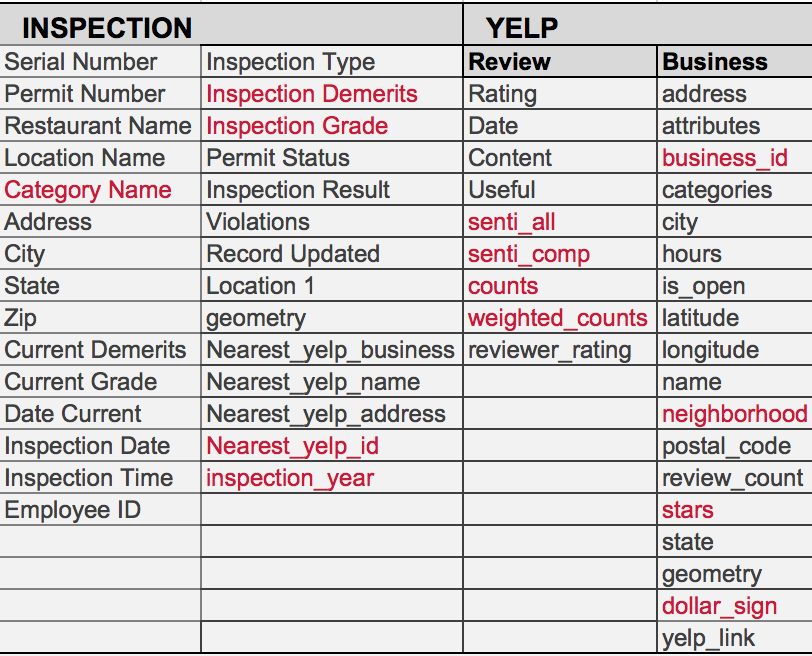
\includegraphics[scale=0.53]{all_features_pic}
    \caption{Feature table of the inspection and Yelp dataset.}
\end{figure}


\subsection*{1.2 Yelp Review Dataset}
Based on the data cleaning result(see explanation in 1.3), we used 630 restaurants information from inspection dataset to get Yelp data. The right half of Figure 1 includes all the features from the dataset. There are two separate datasets, review and business. Business dataset contains basic restaurant information such as their locations, star ratings, expensiveness, etc. Review data is in the unit of per review, so we added weighted features for analyses. 

\subsection*{1.3 Data Fetching and Cleaning}
We initially wanted to use the data from Yelp's Open Data Challenge but we found that the reviews only contain Yelp recommended Reviews. Since we don't know specifically how the reviews were "recommended" by Yelp, the reviews in the Open Data Challenge can potentially be biased. As a result, we decided to web scrap \url{Yelp.com} to get user review data, restaurant information and other related features. Unfortunately, due to time limitation, we were only able to obtain 630 restaurants' review data that matches the restaurants in inspection dataset. 

Reviews are the key information we are interested in to do sentiment analyses. For each restaurant, we obtained the first 40 reviews on their Yelp web page. In addition to capturing review content, we also included dates of the review, "usefulness" of the review evaluated by other users, and review star ratings. General restaurant information such as expensive rating, overall star rating were also obtained by web scraping. As a result of data scraping, we are able to obtain 20,000 review data which is approximately 32 reviews per restaurant. The inspection and Yelp datasets are matched by geographic locations, restaurant names and street name. 

There are two features in business dataset has missing data - neighborhood and dollar sign. We decided to keep dollar sign since only 62 restaurants' data were missing. We 2/3 of missing data with one dollar sign and 1/3 with two based on the dollar sign distribution of the dataset. Neighborhood has a lot more missing data and 2.3 has a detailed explanation on our decision.\newline

\section*{2 Feature Engineering and Descriptive Analysis}
Based on data we acquired, we generated the following features. Due to the nature of \url{Yelp.com}, the main focus of feature engineering is to perform natural language processing on the review texts. We primarily used techniques in sentiment analysis to analyze the users' emotional responses of their dining experience. 
\label{sec:theory}

\subsection*{2.1 Analyzing the Reviews Using VADER Model}
The VADER (Valence Aware Dictionary and Sentiment Reasoner) model is a Python package developed mainly for sentiment analysis (Hutto \& Gilbert, 2014). VADER is based on lexicons of sentiment-related words. Each lexicon is rated to be either positive or negative, along with the valence of positivity and negativity. 

The model first split the text into individual words, and check if any of those words is in the lexicons, and finally produces four sentiment metrics: positive, negative, neutral and compound scores. The first three metrics each represent the proportion of the text that falls into those categories and the compound score is a summary score that ranges from -1 to +1 with negative score representing negative sentiment, vice versa.

In our analysis, we computed a sentiment matrix for every review and averaged the scores for each restaurant. As shown below in Figure 2, there is a slight trend that the negative score correlates positively with the number of demerits occurred in the inspection. 

\begin{figure}[h]
	\centering
    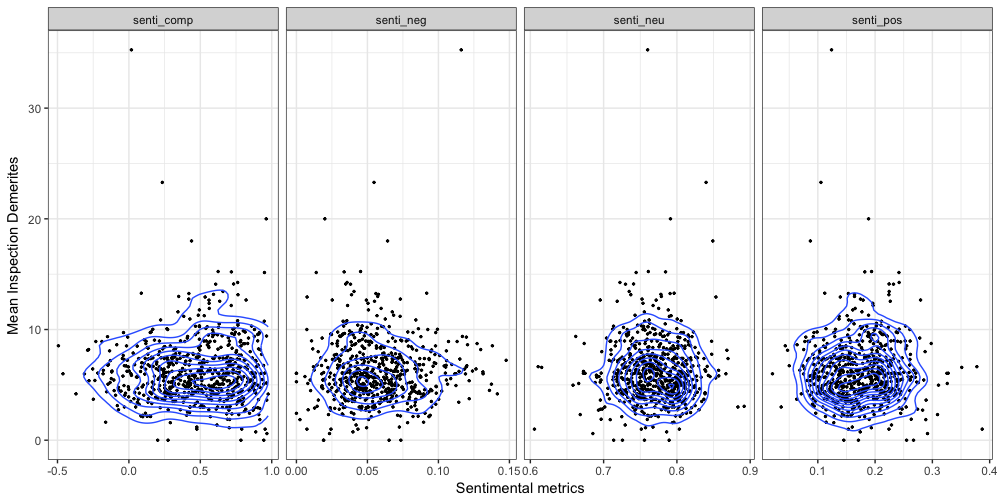
\includegraphics[scale=0.23]{senti_analysis}
    \caption{Sentiment metrics scatter plots (Compounds, Negative, Neutral and Positive).}
\end{figure}

\subsection*{2.2 Keyword Analysis}
In addition to the VADER model, we also defined a set of target keywords that is presumably related to health inspection. As can be seen in Figure 3 and 4, we have 15 subsets of keywords. All words within each subset have similar semantic meaning so that we can account for different users' wording habits. 

\begin{figure}[h]
	\centering
    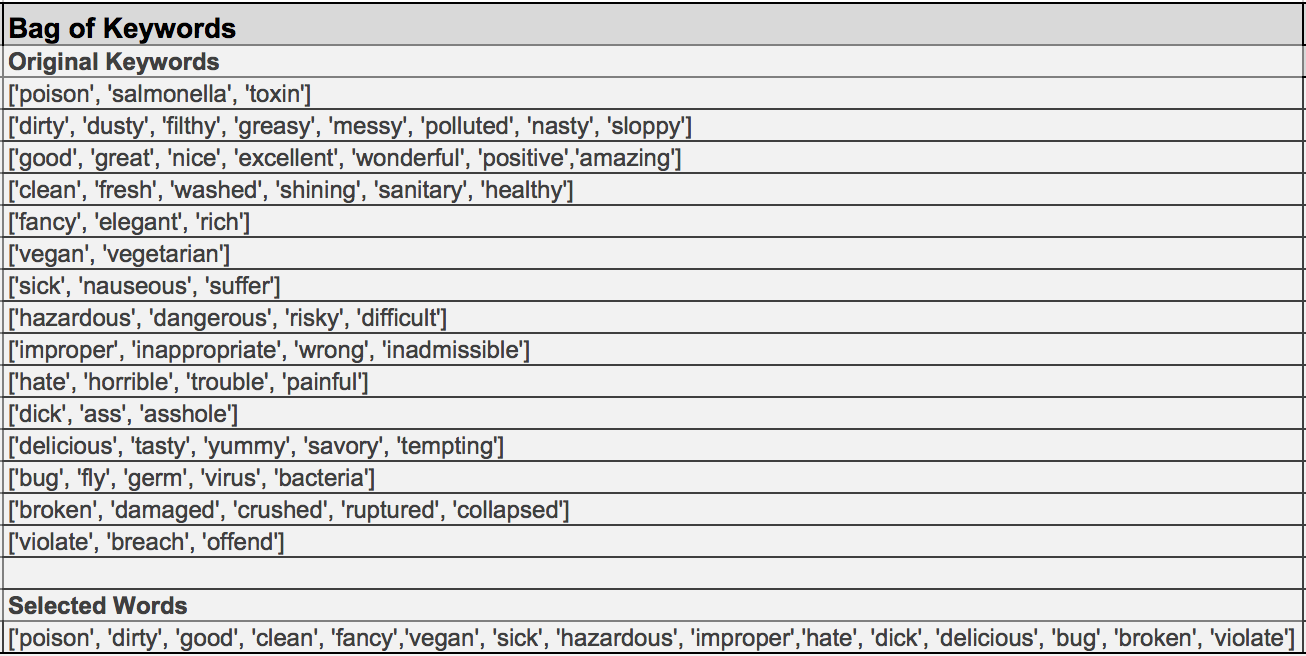
\includegraphics[scale=0.35]{Bag_of_Keywords_pic}
    \caption{Detailed Keyword Set.}
\end{figure}

\begin{figure}[h]
	\centering
    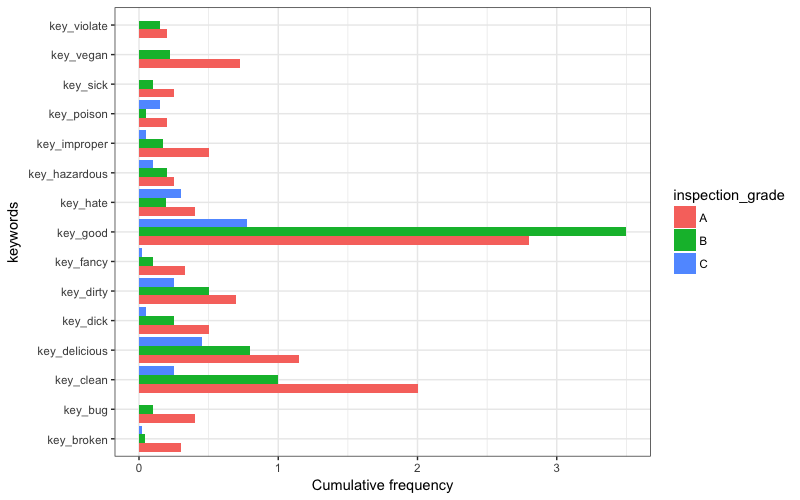
\includegraphics[scale=0.25]{keywords}
    \caption{Cumulative frequencies of 15 key words grouped by the inspection grades.}
\end{figure}

Moreover, we also used the "get\_word\_forms" Python package to get possible verb or adjective forms of the keywords so that we could catch the keywords in different semantic settings. Similar to the VADER analysis, we first divided each review into individual words, then we check if that word is spelled correctly, if not, we found the first 5 most frequent guess of the correct form. Lastly, we checked if any of the words from the review are in the target set. We also multiplied the counts of each subset of the keywords by the number of hits on "usefulness" of the review so that popular reviews get a higher weight in the analysis. After we have the weighted counts for each subset of the keywords, we averaged those counts for each restaurant. 

\subsection*{2.3 Restaurant features}

\begin{itemize}
	\item Neighborhood. The neighborhood information was scrapped from Yelp.com. As shown in Figure 5, certain neighborhoods (e.g. Southeast and East side) has a strong tendency towards larger numbers of demerits, which indicates that neighborhood may be a good predictor. Due to lack of complete information from Yelp, we have 116 missing values in this feature. Since we only have 630 data entries in total and there is no good way to replace this information other than removing them from the analysis. We didn't include this feature in further analysis here, but will include this once we get a larger dataset.
    \item Yelp rating. This is an average representation of Yelp user's ratings on each restaurant. From Figure 6, there is no obvious relationship between ratings and the number of demerits. But the highest rating range has relatively less number of demerits while most outliers have low ratings.
    \item Dollar sign. From Figure 7, most restaurants are among the two lowest price range and the lowest price range has more demerits.
\end{itemize}

\begin{figure}[h]
	\centering
    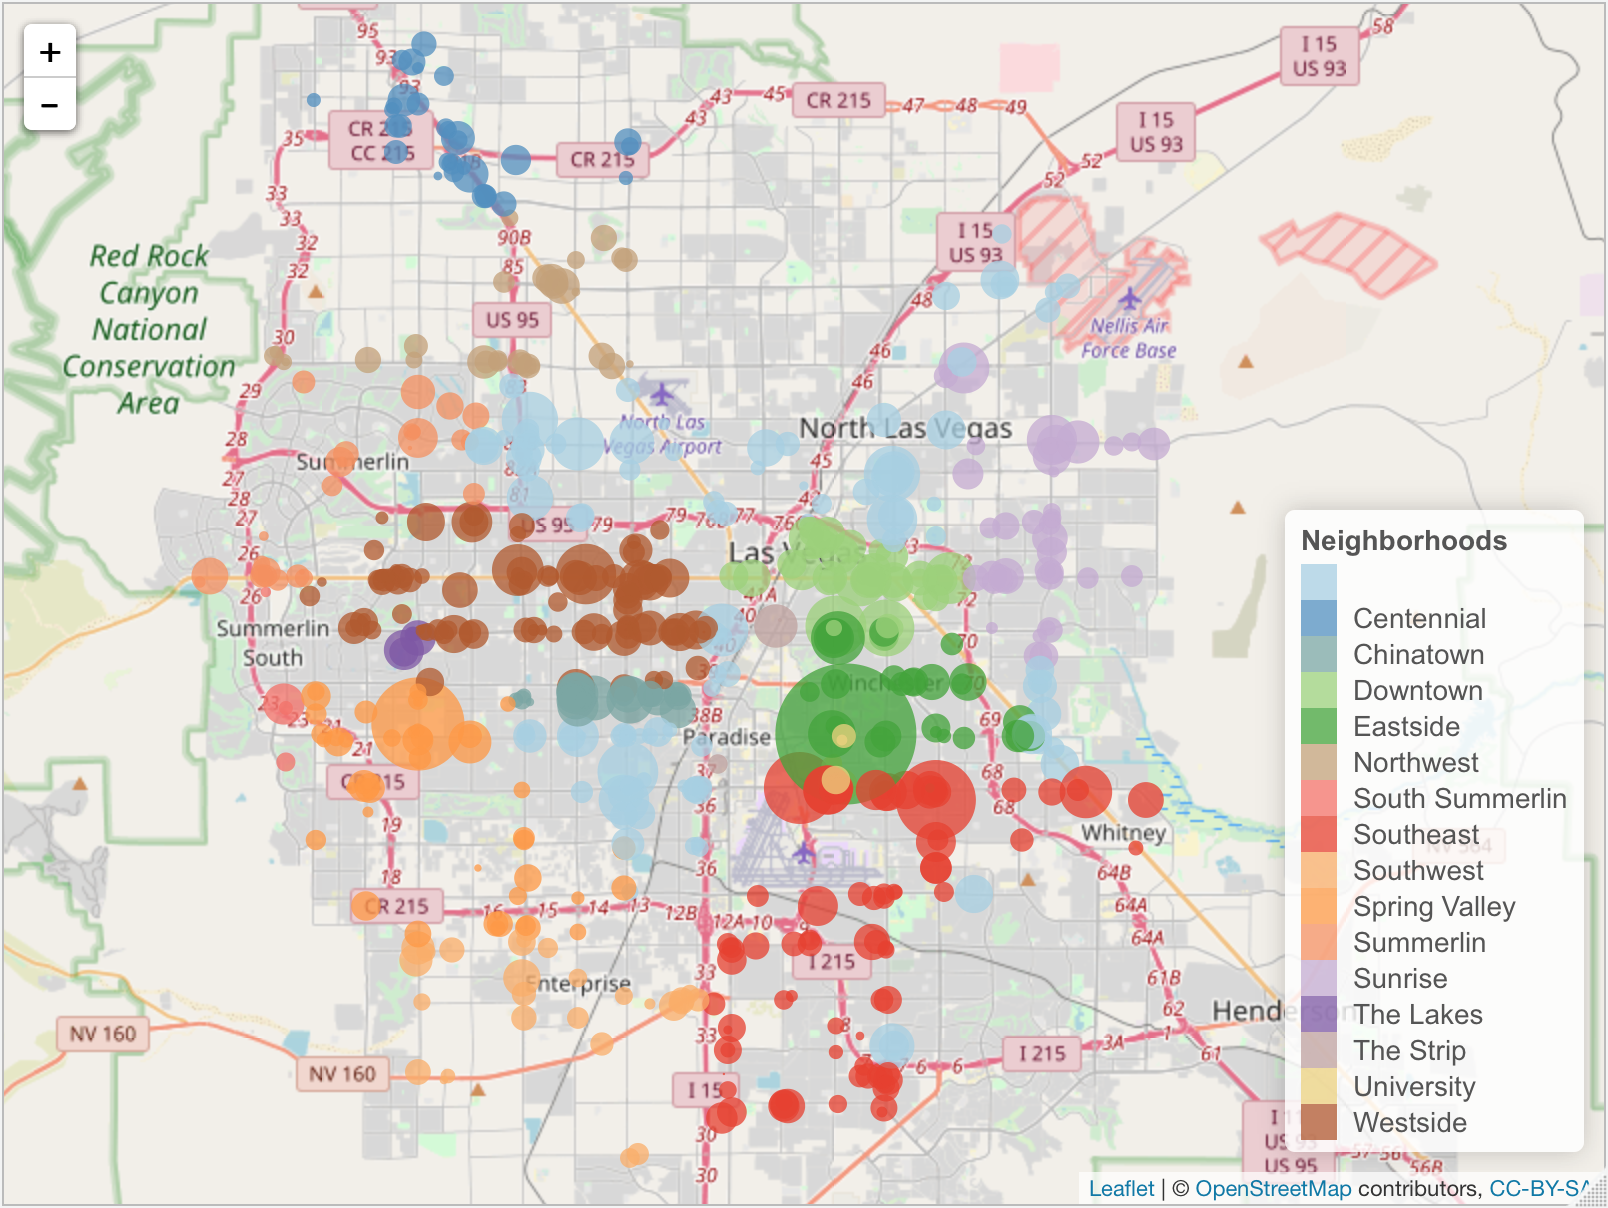
\includegraphics[scale=0.23]{map_demerits}
    \caption{The distribution of restaurants included in Las Vegas. Points are colored by neighborhoods and larger points indicate more demerits.}
\end{figure}

\begin{figure}[h]
	\centering
    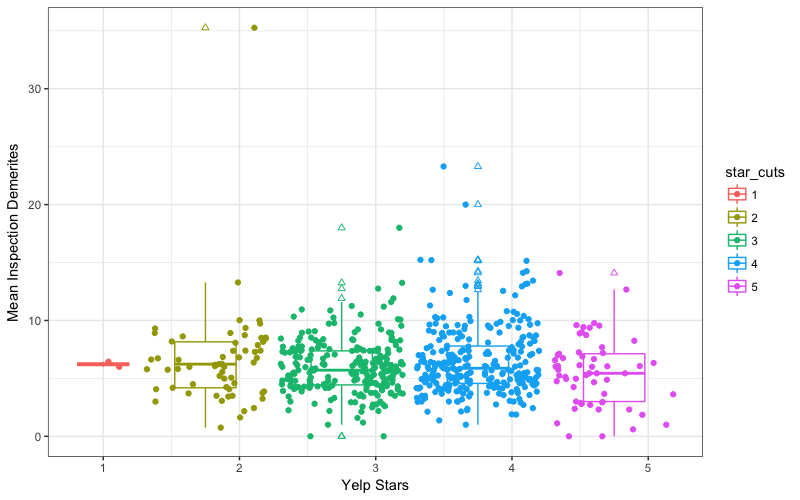
\includegraphics[scale=0.2]{yelp_star}
    \caption{The relationship between overall Yelp rating and number of demerits.}
\end{figure}

\begin{figure}[h]
	\centering
    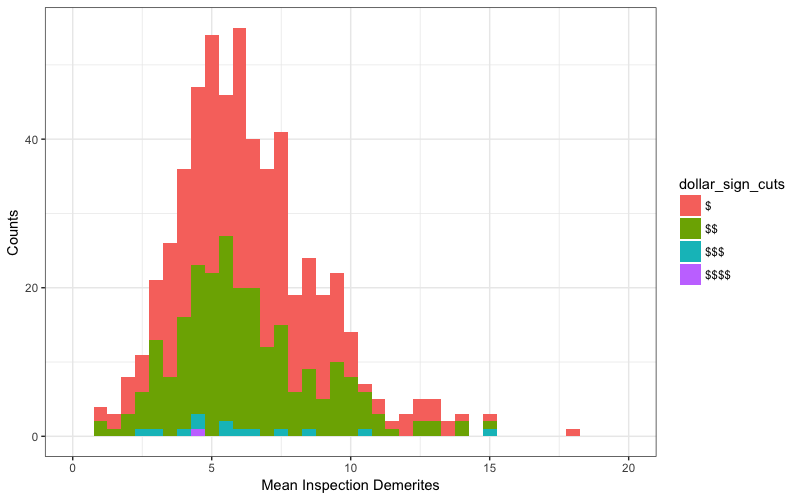
\includegraphics[scale=0.28]{dollar_sign}
    \caption{The relationship between expensiveness rating and number of demerits}
\end{figure}

\section*{3 Preliminary Analysis}
	After feature transformation, we used the features from the table below and tried to fit a linear model to predict the number of demerits occurred in health inspection for each restaurant. The result of a 10-fold cross validation linear model is shown in Figure 8. The model had an average explained variance rate of 7\%. Therefore, our model under-fitted the data. 

\begin{figure}[h]
	\centering
    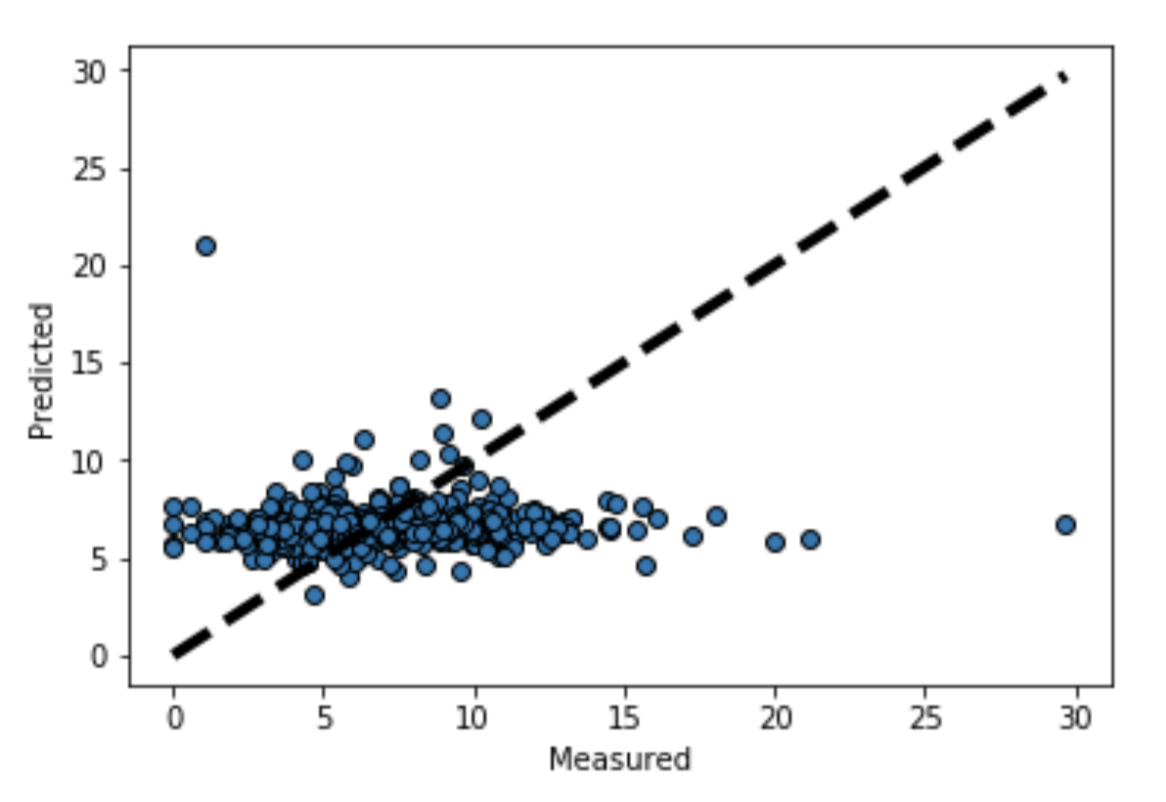
\includegraphics[scale=0.25]{CV_result.png}
    \caption{10-fold Cross Validation Result}
\end{figure}

\section*{4 Future Plans}
Firstly, we need to scrape more data from \url{Yelp.com} that matches the restaurants in the inspection dataset. 

Secondly, after we have more data in hand, we can incorporate the neighborhood in the set of features, and other information such as the demographic information about specific neighborhoods can also serve as potential useful features. 

Lastly, to solve the underfitting problem, we should try to perform some unsupervised learning (e.g. principal component analysis) on the features. Also, we should also build some non-linear (e.g. support vector machines, random forests, etc), or auto-regressive models to find a best fit to our datasets. 

\end{document}